\documentclass[a4paper]{book}
\usepackage{fullpage}

\usepackage[utf8]{inputenc}
\usepackage[T1]{fontenc}
\usepackage[francais]{babel}

\usepackage{latexsym}
\usepackage{fancyhdr}
\usepackage{makeidx}
\usepackage{graphics}
\usepackage{graphicx}
\usepackage{longtable}
\usepackage{moreverb}
\usepackage{listings}

\newcommand{\altarica}{{\sc AltaRica}}

\begin{document}

\title{Master 1, Conceptions Formelles\\
Projet du module \altarica\\
Synthèse (assistée) d'un contrôleur du niveau d'une cuve}

\date{}

\author{Emile ROLLEY \and Gilles SOUTON}

\maketitle

\chapter{Le sujet}
\section{Cahier des charges}

Le système que l'on souhaite concevoir est composé~:
\begin{itemize}
\item d'un réservoir contenant {\bf toujours} suffisamment d'eau pour alimenter l'exploitation,
\item d'une cuve,
\item de deux canalisations parfaites amont reliant le réservoir à la cuve, et permettant d'amener l'eau à la cuve,
\item d'une canalisation parfaite aval permettant de vider l'eau de la cuve,
\item chaque canalisation est équipée d'une vanne commandable, afin de réguler l'alimentation et la vidange de la cuve,
\item d'un contrôleur.
\end{itemize}

\subsection{Détails techniques}

\subsubsection{La vanne}
Les vannes sont toutes de même type, elles possèdent trois niveaux de débits correspondant à trois diamètres d'ouverture~: 0 correspond à la vanne fermée, 1 au diamètre intermédiaire et 2 à la vanne complètement ouverte. Les vannes sont commandables par les deux instructions {\tt inc} et {\tt dec} qui respectivement augmente et diminue l'ouverture. Malheureusement, la vanne est sujet à défaillance sur sollicitation, auquel cas le système de commande devient inopérant, la vanne est désormais pour toujours avec la même ouverture.

\subsubsection{La Cuve}
Elle est munie de $nbSensors$ capteurs (au moins quatre) situés à $nbSensors$ hauteurs qui permettent de délimiter $nbSensors+1$ zones. La zone 0 est comprise entre le niveau 0 et le niveau du capteur le plus bas; la zone 1 est comprise entre ce premier capteur et le second, et ainsi de suite.

Elle possède en amont un orifice pour la remplir limité à un débit de 4, et en aval un orifice pour la vider limité à un débit de 2.  

\subsubsection{Le contrôleur}
Il commande les vannes avec les objectifs suivants ordonnés par importance~:
\begin{enumerate}
\item Le système ne doit pas se bloquer, et le niveau de la cuve ne doit jamais atteindre les zones 0 ou $nbSensors$.
\item Le débit de la vanne aval doit être le plus important possible.
\end{enumerate}

On fera également l'hypothèse que les commandes ne prennent pas de temps, et qu'entre deux pannes et/ou cycle {\em temporel}, le contrôleur à toujours le temps de donner au moins un ordre. Réciproquement, on fera l'hypothèse que le système à toujours le temps de réagir entre deux commandes.

\subsubsection{Les débits}
Les règles suivantes résument l'évolution du niveau de l'eau dans la cuve~:
\begin{itemize}
\item Si $(amont > aval)$ alors au temps suivant, le niveau aura augmenté d'une unité.
\item Si $(amont < aval)$ alors au temps suivant, le niveau aura baissé d'une unité.
\item Si $(amont = aval = 0)$ alors au temps suivant, le niveau n'aura pas changé.
\item Si $(amont = aval > 0)$ alors au temps suivant, le niveau pourra~:
  \begin{itemize}
  \item avoir augmenté d'une unité,
  \item avoir baissé d'une unité,
  \item être resté le même.
  \end{itemize}
\end{itemize}

\section{L'étude}

\subsection{Rappel méthodologique}
Comme indiqué en cours, le calcul par point fixe du contrôleur est exact, mais l'opération de projection effectuée ensuite peut perdre de l'information et générer un contrôleur qui n'est pas satisfaisant. Plus précisemment, le contrôleur \altarica\ généré~:
\begin{itemize}
\item ne garanti pas la non accessibilité des \emph{Situations Redoutées}.
\item ne garanti pas l'absence de \emph{nouvelles situations de blocages}.
\end{itemize}

Dans le cas ou il existe toujours \emph{des situations de blocages ou redoutées}, vous pouvez au choix~:
\begin{enumerate}
\item Corriger manuellement le contrôleur calculé (sans doute très difficile).
\item Itérer le processus du calcul du contrôleur jusqu'à stabilisation du résultat obtenu. 
  \begin{itemize}
  \item Si le contrôleur obtenu est sans blocage et sans situation redoutée, il est alors correct.
  \item Si le contrôleur obtenu contient toujours des blocages ou des situations redoutées, c'est que le contrôleur initial n'est pas assez performant, mais rien ne garanti que l'on soit capable de fournir ce premier contrôleur suffisemment performant.
  \end{itemize}
\end{enumerate}

{\bf Remarque} : Pour vos calculs, vous pouvez utiliser au choix les commandes~:
\begin{itemize}
\item {\tt altarica-studio xxx.alt xxx.spe}
\item {\tt arc -b xxx.alt xxx.spe}
\item {\tt make} pour utiliser le fichier GNUmakefile fourni.
\end{itemize}

\subsection{Le travail a réaliser}
L'étude consiste à étudier le système suivant trois paramètres~:
\begin{enumerate}
\item $nbFailures$~: une constante qui est une borne pour le nombre de vannes pouvant tomber en panne.
\item Le contrôleur initial qui peut être soit {\tt Ctrl}, soit {\tt CtrlVV}.
\item Une éventuelle optimisation pour améliorer le débit aval.
\end{enumerate}

Les questions auxquelles vous devez répondre sont dans le fichier {\tt fichier rapport.tex}. Elles correspondent aux interrogations suivantes~:
\begin{enumerate}
\item Est-il possible de contrôler en évitant les blocages et les situations critiques ?
\item Si oui, donnez quelques caractéristiques de ce contrôleur, si non, expliquez pourquoi.
\item Est-il possible de contrôler en optimisant le débit aval et en évitant les blocages et les situations critiques ?
\item Si oui, donnez quelques caractéristiques de ce contrôleur, si non, expliquez pourquoi.
\end{enumerate}

Vous écrirez vos réponses dans ce même fichier.




\chapter{Le rapport}
Le rapport est sur 20 points.

\section{Processus}

\subsection{Rôle du fichier {\tt GNUmakefile} (1.5 points)}

\begin{itemize}
  \item lignes 1 à 87 : déclaration des variables globales nécessaires pour l'exécution des règles.
  \item règle \texttt{all} : exécute les règles \texttt{sources} et
    \texttt{tank.time} et compile les cibles
    \begin{itemize}
      \item \texttt{sujet.pdf}, \texttt{FD-2021-2022-M1-CC-sujet.tgz},
      \item \texttt{rapport-<user>.pdf}, \texttt{FD-2021-2022-M1-CC-rapport-<user>.tgz},
      \item \texttt{corrige.pdf} et \texttt{FD-2021-2022-M1-CC-corrige.tgz}.
    \end{itemize}
  \item règle \texttt{sources} : exécute \texttt{make all} pour les
    sous-répertoires \texttt{Alt} et \texttt{Spec}.
  \item règle \texttt{tank.time} :
      \begin{enumerate}
          \item Pour chacun des controleurs (\texttt{Ctrl} et \texttt{CtrlVV})
            et pour chaque nombre de défaillance (de 0 à 3), est
            créé un fichier \texttt{tank.alt} . Ce fichier est l'aggrégation de
            l'ensembles des fichiers AltaRica du répertoire \texttt{Alt}.
          \item Les fichiers \texttt{test.alt} et \texttt{test.spe} sont créés
            en remplaçant les différentes \textit{variables} des fichiers
            \texttt{tank.alt} et \texttt{test.spe} par leurs valeurs
            correspondantes -- nombre de pannes, nom du contrôleur, etc...
          \item Les résultats de la commande \texttt{arc} sont ensuite écrits
            dans les fichiers \texttt{Res/*.res} correspondants.
            Cette procédure est répétée jusqu'à stabilisation des résultats (ou
            5 fois maximum dans le cas échéant).
          \item Une fois stabilisé, les fichiers \texttt{test.alt} et
            \texttt{test.spe} sont recréés et exécutéés mais en utilisant la
            version optimisée du contrôleur courant.
          \item Finalement, la commande \texttt{make} est exécutée dans
            tous les sous-répertoires : \texttt{Res} \texttt{Controleurs}
            \texttt{Graphs} \texttt{LaTeX}.
      \end{enumerate}
\end{itemize}

\subsection{Rôle de la constante {\tt nbFailures} et de l'assertion associée (0.5 point)}

La constante \texttt{nbFailures} corresponds au nombre de maximum de vannes
pouvant tombées en pannes simultanément (\texttt{Valve.stucked == 1}). Cette
condition est assurée par l'assertion :
\begin{verbatim}
# ligne 154 tank.alt
nbFailures >= (V[0].stucked + V[1].stucked + V[2].stucked);
\end{verbatim}

Par exemple, si les vannes $0$ et $1$ tombent en pannes :
$$
V[0].stucked + V[1].stucked + V[2].stucked = 1 + 1 + 0 = 2
$$

\section{Résultats avec le contrôleur initial {\tt Ctrl}}
\subsection{Calcul d'un contrôleur}
\subsubsection{Avec 0 défaillance (0.5 point)}
\small{\lstinputlisting{Res/System0FCtrl.res}}
\lstinputlisting{Res/System0FCtrl0F1I.res}
\lstinputlisting{Res/System0FCtrl0F2I.res}

\paragraph{Interprétation des résultats}

Sans défaillance, le contrôleur initial ne vérifie pas l'objectif principal à savoir que
garantir la non accessibilité des situations redoutées ($SR > 0$).
Cependant, après projection, ces situations ne sont plus accessible ($SR = 0$).
De plus le débit de la vanne aval semble avoir été maximisée ($out2 > out1 > out0$), ce qui
valide le second objectif.

La stabilisation est atteinte dès la deuxième itération.

\subsubsection{Avec 1 défaillance (0.5 point)}
\small{\lstinputlisting{Res/System1FCtrl.res}}
\lstinputlisting{Res/System1FCtrl1F1I.res}
\lstinputlisting{Res/System1FCtrl1F2I.res}
\lstinputlisting{Res/System1FCtrl1F3I.res}

\paragraph{Interprétation des résultats}

Avec une défaillance, le contrôleur initial ne garantit pas le maintient du
niveau de la cuve hors des zones critiques ($NC > 0$), cependant, le système ne
peut pas se bloquer ($deadlock = 0$).

Après une première itération le contrôleur calculé à diminué le nombre d'états
où le niveau de la cuve se retrouve en zone critique ($NC = 69$ au lieu de
$93$). En revanche le système peut se bloquer ($deadlock > 0$).

Les itérations suivantes ne modifient pas significativement les résultats.

\subsubsection{Avec 2 défaillances (0.5 point)}

Avec 2 défaillances, le nombre d'états où le niveau de la cuve se retrouve en
zone critique augmente par rapport au système avec une seule défaillance ($SR = NC = 551$).

Après la première itération, le nombre d'états en situation redoutée diminue ($SR = 239$)
mais introduit des situations bloquantes ($deadlock = 239$).
La stabilisation est atteinte à la 4ème itération, cependant, le système ne respecte toujours
par le premier objectif.

\subsubsection{Avec 3 défaillances (0.5 point)}

Avec 3 défaillances, le système ne respecte toujours par le premier objectifs car après
stabilisation $SR = 27$, même si le nombre à diminué par rapport au système avec 2 défaillances,
mais cela s'explique par le fait qu'il y a nécessairement moins d'états accessibles.

\subsection{Bilan avec le contrôleur initial (1 point)}

Le contrôleur initial ne permet de modéliser un système respectant les deux
objectifs seulement si il n'y a pas de défaillances. Il ne permet donc pas de
modéliser un système réaliste et robuste.

\section{Construction d'un contrôleur initial plus performant}
\subsection{Rôle du composant {\tt ValveVirtual}(2 points)}
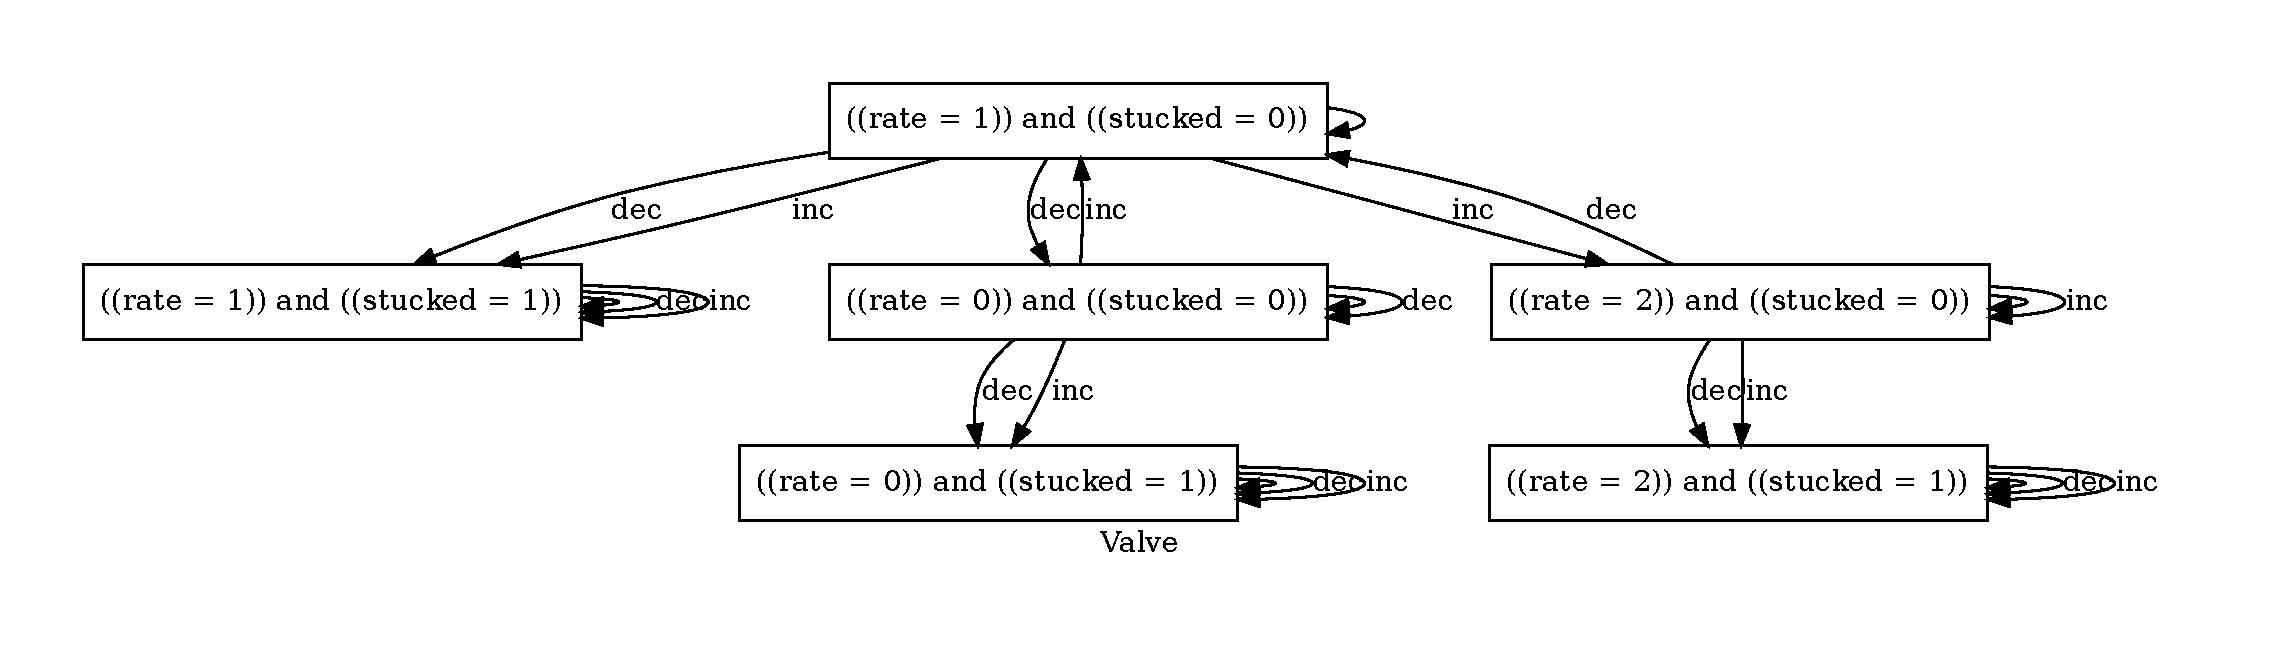
\includegraphics[height=.2\textheight,width=.5\textwidth]{Graphs/Valve-modes.pdf}
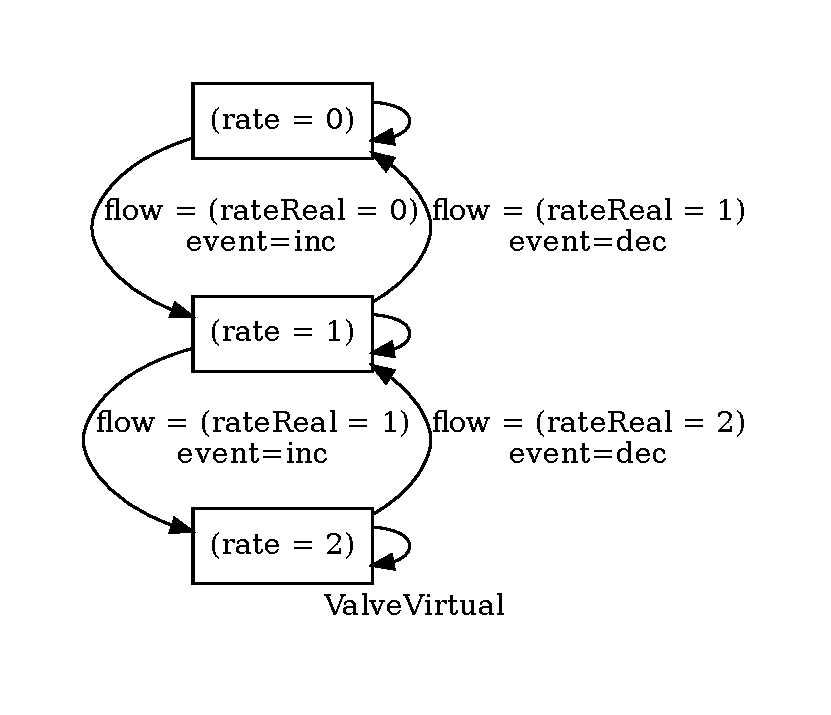
\includegraphics[height=.2\textheight,width=.5\textwidth]{Graphs/ValveVirtual-modes.pdf}

Le composant \texttt{ValveVirtual} est la représentation en droit d'une valve
physique. Elle permet donc de simuler le fonctionnement et l'évolution d'une
valve \textit{parfaite}, c'est-à-dire, sans contrainte de l'environnement :
elle ne peut donc pas tomber en panne.

Sa sémantique est la suivante :
\begin{itemize}
  \item si les variables \texttt{rate} et \texttt{reateReal} coincïdent, alors l'évènement \texttt{dec} (resp. \texttt{inc})
    permet de décrementer (resp. incrémenter) la valeur de \texttt{rate}.
  \item sinon, dès lors que les variables \texttt{rate} et \texttt{rateReal} se
    désynchronisent, cela signifie que la valve physique est tombée en panne : la valve virtuelle
    n'est alors plus utilisable.
\end{itemize}

\subsection{Rôle du composant {\tt CtrlVV} (4 points)}
% A COMPLETER en expliquant les mécanismes mis en oeuvre, leurs rôles et les
% avantages de ce contrôleur par rapport au précédent CtrlVV.

\section{Résultats avec le contrôleur {\tt CtrlVV}}
\subsection{Calcul d'un contrôleur}
\subsubsection{Avec 0 défaillance (0.5 point)}
\small{\lstinputlisting{Res/System0FCtrlVV.res}}
\lstinputlisting{Res/System0FCtrlVV0F1I.res}
\lstinputlisting{Res/System0FCtrlVV0F2I.res}

\paragraph{Interprétation des résultats}
% A COMPLETER

\subsubsection{Avec 1 défaillance (0.5 point)}
\small{\lstinputlisting{Res/System1FCtrlVV.res}}
\lstinputlisting{Res/System1FCtrlVV1F1I.res}
\lstinputlisting{Res/System1FCtrlVV1F2I.res}
\lstinputlisting{Res/System1FCtrlVV1F3I.res}
\lstinputlisting{Res/System1FCtrlVV1F4I.res}

\paragraph{Interprétation des résultats}
% A COMPLETER

\subsubsection{Avec 2 défaillances (0.5 point)}
\small{\lstinputlisting{Res/System2FCtrlVV.res}}
\lstinputlisting{Res/System2FCtrlVV2F1I.res}
\lstinputlisting{Res/System2FCtrlVV2F2I.res}
\lstinputlisting{Res/System2FCtrlVV2F3I.res}

\paragraph{Interprétation des résultats}
% A COMPLETER

\subsubsection{Avec 3 défaillances (0.5 point)}
\small{\lstinputlisting{Res/System3FCtrlVV.res}}
\lstinputlisting{Res/System3FCtrlVV3F1I.res}
\lstinputlisting{Res/System3FCtrlVV3F2I.res}
\lstinputlisting{Res/System3FCtrlVV3F3I.res}

\paragraph{Interprétation des résultats}
% A COMPLETER

\subsection{Bilan avec le contrôleur CtrlVV (1 point)}
% A COMPLETER

\section{Une première optimisation des contrôleurs pour améliorer le débit aval}
\subsection{Une optimisation basée sur les priorités (1 point)}
\small{\lstinputlisting{ControleursOpt/Optimisation.alt}}
L'optimisation mise en place défini un ordre de priorité sur les différentes
actions sur les vannes. En particulier, sur la vanne aval : $inc > nop > dec$.
Cela forcera donc à choisir les actions maximisant le débit de la vanne aval,
en effet, l'action incrémentant le débit est prioritaire par rapport aux deux
autres et l'action de ne pas modifier le débit est prioritaire à celle le
diminuant.

\subsection{Calcul des contrôleurs optimisés avec {\tt CtrlVV}}
\paragraph{Avec 0 défaillance}\ \\
box{\small{\lstinputlisting{Res/System0FCtrlVV0F2I_opt.res}}}


\paragraph{Avec 1 défaillance}\ \\
box{\small{\lstinputlisting{Res/System1FCtrlVV1F4I_opt.res}}}


\paragraph{Avec 2 défaillances}\ \\
box{\small{\lstinputlisting{Res/System2FCtrlVV2F3I_opt.res}}}


\paragraph{Avec 3 défaillances}\ \\
box{\small{\lstinputlisting{Res/System3FCtrlVV3F3I_opt.res}}}


\subsection{Bilan avec la première optimisation du contrôleur CtrlVV (1 point)}

Sans défaillance, tous les objectifs énnoncés pour le contrôleur sont respectés :
\begin{itemize}
  \item $SR = 0$, assure que le system ne peut pas se bloquer ($deadlock = 0$)
    et que le niveau de la cuve ne dépasse jamais les niveau critiques ($NC =
    0$),
  \item $out2 > out1 > out0$, démontre que le débit de la vanne aval est
    maximisé, c'est accentué par le fait que le débit n'est décrementé qu'une
    seule fois ($dec21 = 1 \wedge dec10 = 0$).
    (TODO: est-ce suffisant pour assurer que le débit aval est maximisé ?)
\end{itemize}


Avec une défaillance, tous l'objectif prioritaire énnoncé pour le contrôleur est respecté car $SR = 0$, cependant,
pour l'optimisation du débit aval : TODO: comprendre CCoupGagnant.

A partir de 2 défaillances, le système ne se bloque pas et la niveau de la cuve
ne dépasse pas les niveaux critiques ($SR = 0$), mais cela à un coup car le
système ne possède plus que deux états ($any\_s = 2$).


\section{Une deuxième optimisation (3 points)}
Il est possible d'obtenir de meilleurs résultats que les précédents par au moins deux façons.
\begin{enumerate}
\item En utilisant un meilleur ordre pour les priorités entre événements.
\item En introduisant cet objectif dans le système de calcul de point fixe des actions du contrôleur.
\end{enumerate}

Vous devez proposer une des deux optimisations conduisant à une solution dans laquelle le débit de la vanne aval est le moins souvent possible décrémenter, voire jamais. Pour cela, vous pouvez~:
\begin{itemize}
\item Meilleur ordre sur les événements.
  \begin{enumerate}
  \item Modifier le fichier \texttt{ControleursOpt/Optimisation.alt}.
  \item Faites \texttt{make}.
  \item Quand vos résultats sont satisfaisants, notez les, puis copiez votre fichier dans \texttt{ControleursOpt/Optimisation-2.alt}.
  \item Remettez le fichier \texttt{ControleursOpt/Optimisation.alt} d'origine.
  \item Faites \texttt{make}.
  \end{enumerate}
\item Meilleur système d'équations au point fixe.
  \begin{enumerate}
  \item Modifier le fichier \texttt{Spec/System.spe}.
  \item Faites \texttt{make}.
  \item Quand vos résultats sont satisfaisants, notez les, puis copiez votre fichier dans \texttt{Spec/System-2.spe}.
  \item Remettez le fichier \texttt{Spec/System.spe} d'origine.
  \item Faites \texttt{make}.
  \end{enumerate}
\end{itemize}

\paragraph{Le nouvel ordre}\ \\
\small{\lstinputlisting{ControleursOpt/Optimisation-2.alt}}
% A COMPLETER en décrivant les résultats obtenus

\paragraph{Le nouveau système d'équations}\ \\
\small{\lstinputlisting[texcl]{Spec/System-2.spe}}
% A COMPLETER en décrivant les résultats obtenus

\section{Conclusion sur la synthèse de contrôleur (1 point)}
% A COMPLETER

\end{document}
